\section{Strategy}
\label{sec:db:strategy}

This analysis is a completely general search for a particle of unknown mass and lifetime, the
following chapter outlines the strategy employed; exhaustive details can be found in
\Ref{Williams:2015xfa}.
Broadly, the search involves a fully frequentest scan of the dimuon invariant mass spectrum from
\btokstrmumu for an excess of events consistent with \dbtomumu.
The scan is performed in two dimensions, namely: mass and lifetime.

Firstly, an explanation of the search in the mass dimension will be presented, and then extended to
to deal with the lifetime dimension.


\subsection{Searching in the mass dimension}
A scan in mass is performed where the test mass, \mass{t}, is incremented in steps of
$\tfrac12\sigmam$, where $\sigmam$ is the local mass resolution defined at \mass{t}, and is in the
range $1\lesssim\sigmam\lesssim6\mev$.
At each \mass{t} a signal region is defined as $|m-\mass{t}<2\sigmam$ and a sideband, or
background, region is defined as $3<|m-\mass{t}|<(2x+3)\sigmam$, where
$x$ defines the width of the sideband regions with respect to the signal region.
The idea of constructing the two regions is to use the sideband regions to estimate the background
contribution in the signal window.

At each mass point in the search the number of events in the signal region, $n_s$, and the number
of events in the background events, $n_b$, are counted.
If the background is linear --- on average --- in the local mass region, then
$\langle n_s\rangle=\langle n_b\rangle/2$ if there is no signal contribution.
However, if there is a signal contribution from a decaying \db then $n_s=s+b$, where $s$ is the
number of signal events, and $b$ is the background in the signal region, which is estimated from the
sideband regions.
Thus, one can construct a likelihood
\begin{equation}
  \mathcal{L}(n_s, n_b | s, b) =
  \mathcal{P}(n_s, s+b) \cdot
  \mathcal{P}(n_b, xb),
  \label{eq:db:like1}
\end{equation}
where $\mathcal{P}(n, \lambda)$ is the probability of observing $n$ from a Poisson distribution
parameterize by $\lambda$.
This just parameterizes the likelihood of the background estimate from the sidebands fluctuating to
the observed number of events in the signal region.
Twice, so far, the local linearity of the background has been mentioned as the sole assumption,
this is important to bare in mind throughout.

The problem with \Eq{eq:db:like1} is that, while $x$ has been chosen, deviations from a linear
background distribution mean that the actual sideband size with respect to the signal region is not
$x$.
Rather, the actual scaling factor is some $y$, with some uncertainty $\sigma_y$.
This can be accounted for by including an additional term in the likelihood
\begin{equation}
  \mathcal{L}(n_s, n_b, x | s, b, y) =
  \mathcal{P}(n_s, s+b) \cdot
  \mathcal{P}(n_b, yb) \cdot
  \mathcal{G}(y,x,\sigma_y),
  \label{eq:db:like2}
\end{equation}
where $\mathcal{G}(n, \mu, \sigma)$ is the probability of observing $n$ given a Gaussian
distribution with a mean, $\mu$, and standard deviation, $\sigma$.

The dimuon background from the \sm decay of \btokstrmumu is expected to be locally-linear, in the
absence of resonances, to better than $1\pc$ over the entire mass range.
However, including resonances in the model lead to significant deviations from linearity.
The magnitude of the deviation is dependent upon the width of a resonance, $\Gamma$, the size of it
relative to the local background distribution, and the value of $x$.
Wide resonances, $\Gamma\gtrsim20\sigmam$, are sufficiently wide not as to be problematic even if
they dominate the local background distribution.
Conversely, narrow resonances where $\Gamma\lesssim5\sigmam$ lead to significant deviations from a
locally-linear background and must, therefore, be vetoed.
Intermediate resonances, $5\lesssim\Gamma\lesssim20\sigmam$, must be considered on a case-by-case
basis since they are only troublesome if they account for a large fraction of the local background.
For this analysis these ranges roughly translate to requiring that resonances with $\Gamma<25\mev$
will be vetoed, while those with $\Gamma>100\mev$ shall be ignored.

Table~\ref{tab:db:bkg} lists a number of mesons, $X$, that decay to a dimuon final state and could
contribute as background to the decay \decay{\Bd}{\Kstarz\mumu}.
The \phii, \jpsi, and \psitwos mesons have the highest branching fraction, and are also among the
narrowest resonances; falling into the $\Gamma\lesssim5\sigmam$ region, and are therefore vetoed.
The remaining resonances are broad and contribute to the dimuon structures at low mass, it is shown
in \Ref{Williams:2015xfa} that the local-linearity approximation is accurate to \approx$5\pc$.
Therefore, below the mass of the \jpsi the values of $x=5$ and $\sigma_y=0.05$ are used.

\begin{table}
    \caption{
      Some particles properties for mesons which decay into a dimuon pair, and the branching
      fraction for the relevant decays; all numbers are taken from Ref.~\cite{PDG2014}.
      Central values of mass and width are given in MeV.
    }
    \label{tab:db:bkg}
    \begin{center}
      %\begin{tabular*}{\textwidth}{lrc @{\extracolsep{\fill}} r @{\extracolsep{\fill}} rc}\toprule
      \scalebox{0.9}{
    \begin{tabular*}{1.1\textwidth}{lrc @{\extracolsep{\fill}} r @{\extracolsep{\fill}} r
      @{\extracolsep{\fill}} c}
      \toprule
      \cellc{$X$} & \cellc{$m$} & \cellc{$\Gamma$}
      & \cellc{$\BF(\decay{\Bd}{\Kstarz X})$}
      & \cellc{$\BF(\decay{X}{\mumu})$}
      & \cellc{$\BF_\mathrm{tot}(\decay{\Bd}{\Kstarz\mumu})$}
      \\\midrule
      ${\eta}$        & $\pz547.9$ & $\pzz0.001$
      & $(1.59\pm0.10)\e{-5}$
      & $(5.8\pz\pm0.8\pz)\e{-6}$
      & $(9.2\pm1.4)\e{-11}$
      \\
      ${\rho}$   & $\pz775.3$ & $147.8\pzz$
      & $(3.9\pz\pm1.3\pz)\e{-6}$
      & $(4.55\pm0.28)\e{-5}$
      & $(1.8\pm0.6)\e{-10}$
      \\
      ${\omega}$ & $\pz782.7$ & $\pzz8.5\pzz$
      & $(2.0\pz\pm0.5\pz)\e{-6}$
      & $(9.0\pz\pm3.1\pz)\e{-5}$
      & $(1.8\pm0.8)\e{-10}$
      \\
      ${\phi}$  &   $1019.5$ & $\pzz4.3\pzz$
      & $(1.00\pm0.05)\e{-5}$
      & $(2.87\pm0.19)\e{-4}$
      & $(2.9\pm0.2)\e{-\pz9}$
      \\
      ${\Dz}$         &   $1864.8$ & $\pz10.1\pzz$
      & $(4.2\pz\pm0.6\pz)\e{-5}$
      & $<6.2\e{-9}$
      & \makebox[\widthof{$(2.9\pm0.2)\e{-\pz9}$}][r]{$<2.6\e{-14}$}
      \\
      \jpsi & $3096.9$ & $\pzz0.093$
      & $(5.96\pm0.03)\e{-2}$
      & $(1.32\pm0.06)\e{-3}$
      & $(7.9\pm0.4)\e{-\pz5}$
      \\
      \psitwos & $3686.1$ & $\pzz0.299$
      & $(7.9\pz\pm0.9\pz)\e{-3}$
      & $(6.0\pz\pm0.4\pz)\e{-4}$
      & $(4.7\pm0.6)\e{-\pz6}$
      \\
      \bottomrule
    \end{tabular*}
  }
  \end{center}
\end{table}

Resonances that lie in the grey area, $5\lesssim\Gamma\lesssim20\sigmam$, are various \ccbar states
with masses above the mass of the \psitwos.
For example, there is contribution from the $\psi(4160)$ which was observed by \lhcb in the decay
\decay{\Bd}{\Kp\mumu}~\cite{LHCb-PAPER-2013-039}.
All known charmonium resonances in this region are wide,
$\Gamma\sim70\mev$, and are dealt with by reducing the size of the sidebands to $x=1$ and
increasing the value of $\sigma_y$ to 0.1.
A summary of the values of $x$ and $\sigma_y$ are given in \Table{tab:db:xsigmay}.

Reference~\cite{Williams:2015xfa} also investigates the effect of interference effects between
\btokstrmumu and \decay{\Bd}{\Kstarz\rho(770)}, where \decay{\rho(770)}{\mumu}.
Considering that the branching fraction of the $\rho(770)$ decay is so small that less than one
event is to be expected in the data sample used in this analysis, interference effects could
produce a deviation in from local linearity.
This deviation could be a maximum of $5\pc$, which is accounted for in the choice of $\sigma_y$.

\begin{table}
  \caption[Values of $x$ and $\sigma_y$ used]
  {
    Values of $x$ and $\sigma_y$ used above and below the \jpsi mass.
  }
  \label{tab:db:xsigmay}
  \begin{center}
    \begin{tabular}{ccc}\toprule
      Region & $x$ & $\sigma_y$ \\\midrule
      $\mass{\mumu}<\mass{\jpsi}$ & 5 & 0.05 \\
      $\mass{\mumu}>\mass{\jpsi}$ & 0 & 0.10 \\
      \bottomrule
    \end{tabular}
  \end{center}
\end{table}

The contribution from the decay \decay{\phi}{\mumu} is removed by excluding dimuon candidates in
the range $1000<\mass{\mumu}<1040\mev$.
Vetoed regions for the \jpsi and \psitwos are calculated using a theoretical model, in
Ref.~\cite{Bobeth:2011nj}, to account for the interference effects between the \jpsi, \psitwos and
the non-resonant dimuon component.
This model is used to model the shape of these two large \ccbar contributions to the \mumu final
state with different phases between resonant and non-resonant components, and then this is
convolved with a Gaussian to account for the resolution of the \lhcb detector, as shown in
\Fig{fig:db:ccbar}.
These \glspl{PDF} are used to calculate the regions around the \jpsi and \psitwos where the
background is locally linear to better than $5\pc$ for various values of $x$.
This method results in veto regions which are very similar to those used in
\Ref{LHCb-CONF-2015-002}, except that the upper boundary of the \psitwos veto is extended to cover
the $\psi(3770)$.
All the veto regions for narrow resonances decaying via \decay{X}{\mumu}, are summarized in
\Table{tab:db:narrow}.

\begin{figure}
  \begin{center}
    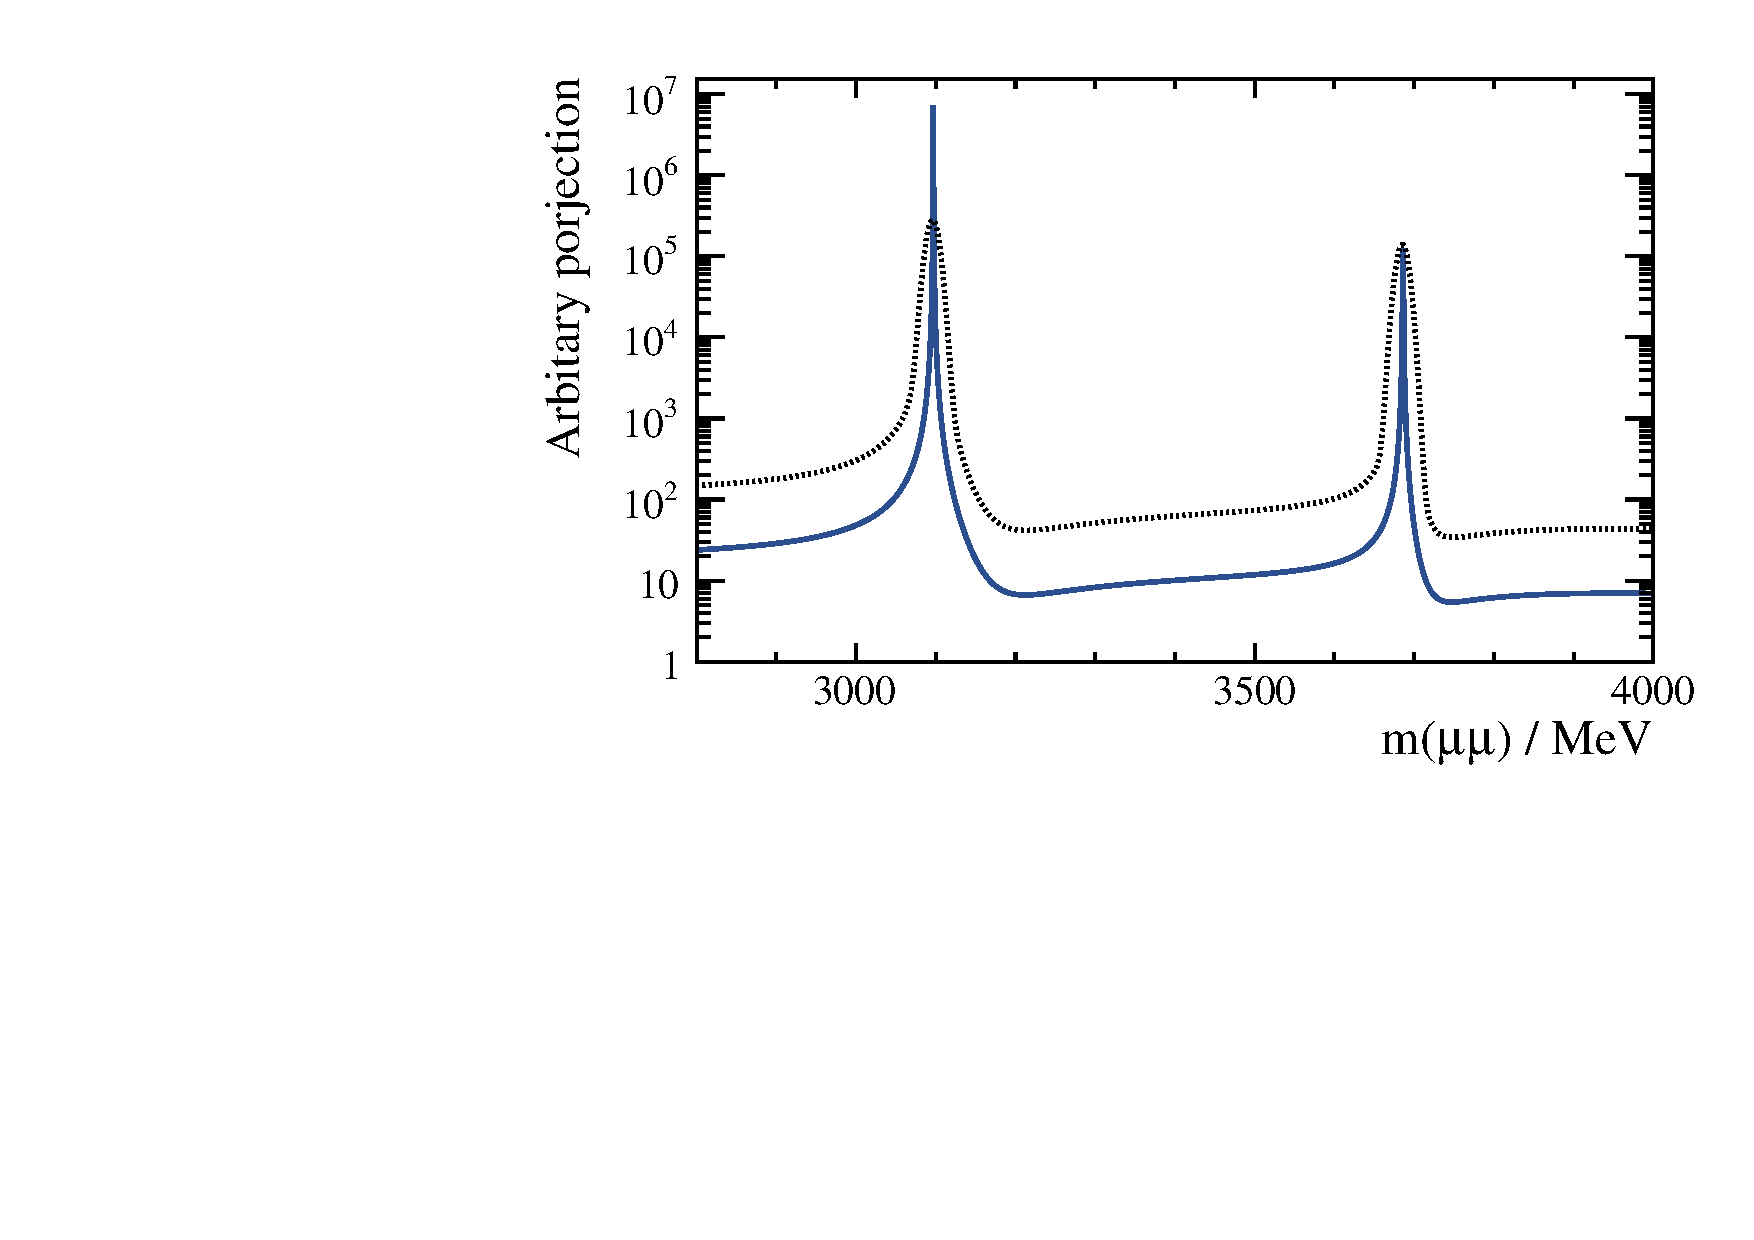
\includegraphics[width=0.48\textwidth]{ccbar_0_0}
    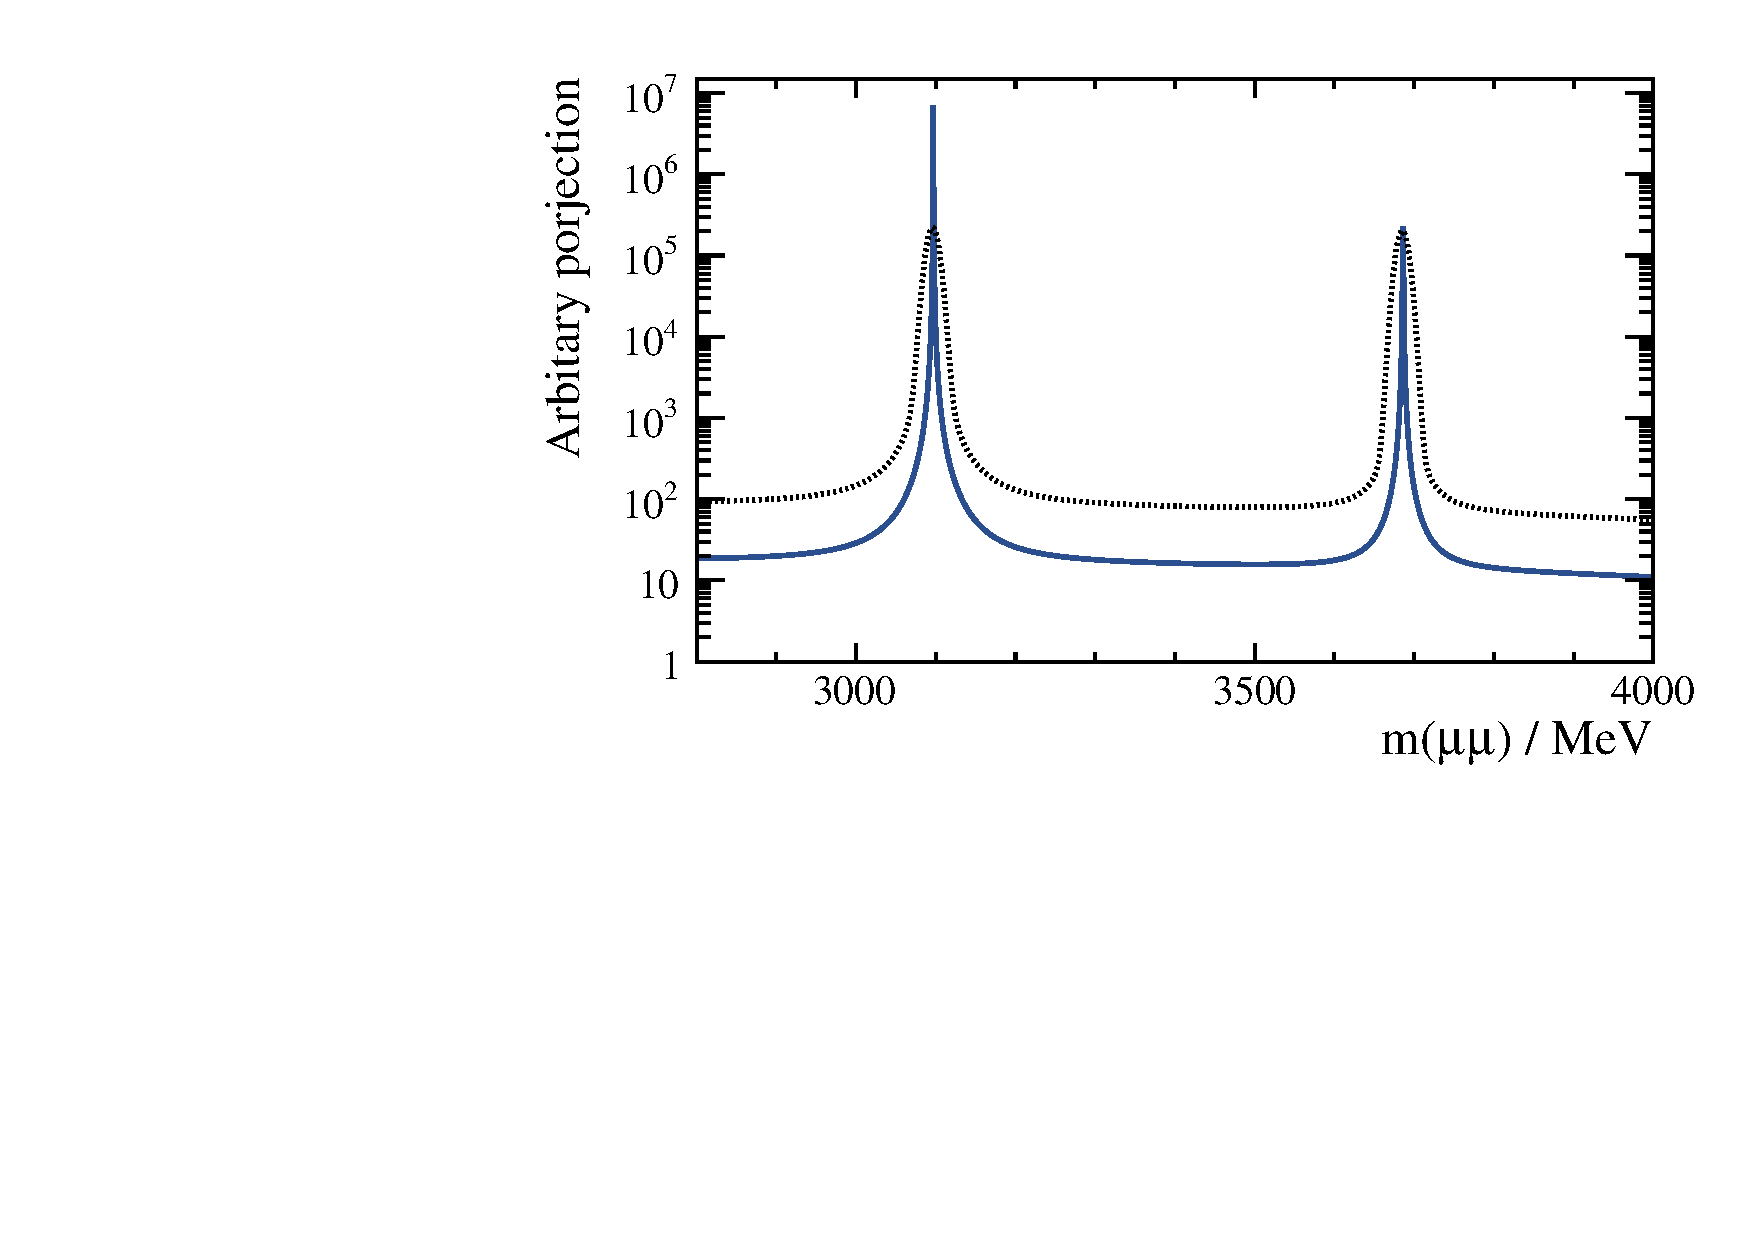
\includegraphics[width=0.48\textwidth]{ccbar_1_57_1_57}
    \caption{
      PIG
    }
    \label{fig:db:ccbar}
  \end{center}
\end{figure}


\begin{table}
  \caption{
    DOGS
  }
  \label{tab:db:narrow}
  \begin{center}
    \begin{tabular}{lc}\toprule
      Resonance(s) & Vetoed region (MeV) \\\midrule
      \phii & $1000<\mass{\mumu}<1040$ \\
      \jpsi & $2960<\mass{\mumu}<3204$ \\
      \psitwos, $\psi(3770)$ & $3614<\mass{\mumu}<3875$ \\
      \bottomrule
    \end{tabular}
  \end{center}
\end{table}









%Narrow resonances, falling in the $\Gamma\lesssim5\sigmam$ region are removed:
%these include the \phii, \jpsi, and \psitwos.
%The decay \decay{\phi}{\mumu} is removed by excluding dimuon candidates in the range
%$1000<\mass{\mumu}<1040\mev$.
%Charmonuim resonances are vetoed using



%The largest deviations from a locally-linear background are at the $5\%$ level, which is
%natrually accounted for by setting \






%Practically, the resonances that must be removed from the background are the \phi, \jpsi, \psitwos

The profile likelihood, $\Lambda$, is defined as
\begin{equation}
  \Lambda(s|n_s,n_b) =
  \frac
  {\mathcal{L}(s, \hat{b}(s), \hat{y}(s) | n_s, n_b, x)}
  {\mathcal{L}(\hat{s}, \hat{b}, \hat{y} | n_s, n_b, x)},
  \label{eq:profilelike1}
\end{equation}
where $\hat{s}$, $\hat{b}$, and $\hat{y}$ are chosen to maximize the likelihood; the functions
$\hat{b}(s)$ and $\hat{y}(s)$ maximize the likelihood for a given $s$.
The solutions to these parameters can be calculated analytically, with few assumptions made,
and thus the likelihood can be minimized with minimal computational power.
The profile likelihood can then be formed in the same way as in \Eq{eq:profilelike1} and solved
analytically.


\subsection{Searching in the lifetime dimension}
Sensitivity to the lifetime of \db is introduced by splitting the data at each \mass{t} into two
regions: a prompt region defined by $\tau<3\sigmat$, and a displaced region defined by
$\tau>3\sigmat$; where \sigmat is defined to be the local lifetime resolution.
The joint likelihood, which takes account of the two lifetime regions, is then the product of the
individual likelihoods:
\begin{align}
  \mathcal{L}(n^p_s, n^p_b, n^d_s, n^d_b, x | s^p, b^p, y^p, s^d, b^d, y^d) =&
  \mathcal{L}(n^p_s, n^p_b, x | s^p, b^p, y^p)\\\nonumber
  \times\mathcal{L}(n^d_s, n^d_b, x | s^d, b^d, y^d),
  \label{eq:db:liketau}
\end{align}
where the superscripts $p$ and $d$ indicate the prompt and displaced regions, respectively.

The information supplied by the addition of two bins in the lifetime dimension is approximately
optimal for all \db lifetimes, except for when $\tau\sim3\sigmat$.
In this case, it is marginally more optimal to include shape information; but this introduces
significantly more complications to the analysis and there is no reason to believe that the \db has
a lifetime $\tau\sim3\sigmat$ \emph{a priori}, and therefore shape information is not used.




\subsection[Calculation of $p$-value]
{Calculation of $\boldsymbol{p}$-value}
For each \mass{t} a $p$-value is calculated using the
Because there are $\mathcal{O}(1000)$ test masses, each of which is not completely independent the
look elsewhere effect must be accounted for.
To do this the minimum local $p$-value is translated into a global $p$-value using a trials factor
which is calculated using an ensemble of toys.

After the $p$-value at each \mass{t} is calculated, the region in which the lowest $p$-value
consistent with zero signal will be isolated and removed from the sample; leaving data which
which is entirely background.
This is assuming that there is only one \np particle that can be observed in this analysis.
The remaining background-like distribution is then turned into a \PDF --- where the region that is
removed is interpolated across --- from which toy datasets can be generated.
In order to obtain a trials factor, 10 million toy datasets are generated, and the minimum
$p$-value is plotted in a cumulative distribution, such that the $y$ axis is the fraction of toy
datasets with a minimum $p$-value...











\subsection{Limits}
Upper limits will be set as a function of \mass{\db} and \lifetime{\db}.
This requires a modification to the likelihood function to

for each \lifetime there is a relationship between the number of signal events in the prompt and
displaced regions

gaussian term is added to account for uncertainty (due to eff) in frac of signal expected in prompt
and displaced regions

another Gaussian term is added to the likelihood to account for uncertainty in the abs eff scale of
the signal

likelihood for each \mass{t}, $\tau$
\begin{align}
  \like\big(n_s^p, n_b^p, n_s^d, n_b^d, x, \tau | \dots\big) =
   &\like\big(n_s^d, n_b^d, x | \varepsilon\cdot s\cdot f,b^p,y^p\big) \\\nonumber
   &\times\like\big(n_s^p, n_b^p, x | \varepsilon\cdot s\cdot(1-f),b^d,y^d\big)\\\nonumber
   &\times\mathcal{G}\big(f, f_\mathrm{sim}(\tau),\sigma(f)\big)
   \times\mathcal{G}\big(\varepsilon, \varepsilon_\mathrm{sim}(\tau),\sigma(\varepsilon)\big)
\end{align}
where f is the fraction of signal events in the prompt region, with expected value from simulation
being $f_\mathrm{sim}$ with uncertainty $\sigma(f)$, $\varepsilon$ is the efficiency (relavtive to
normalization channel) with expected valu from simulation $\varepsilon_\mathrm{sim}$ and
uncertainty $\sigma(\varepsilon)$.

Limits are set by scanning the profile likelihood using the same method, including the likelihood
given



















